%%%%%%%%%%%%%%%%%%%%%%%%%%%%%%%%%%%%%%%%%%%%%%%%%%%%%%%%%%%%%%%%%%%%%%
%%  disstemplate.tex, to be compiled with latex.		     %
%%  08 April 2002	Version 4				     %
%%%%%%%%%%%%%%%%%%%%%%%%%%%%%%%%%%%%%%%%%%%%%%%%%%%%%%%%%%%%%%%%%%%%%%
%%								     %
%%  Writing a Doctoral Dissertation with LaTeX at		     %
%%	the University of Texas at Austin			     %
%%								     %
%%  (Modify this ``template'' for your own dissertation.)	     %
%%								     %
%%%%%%%%%%%%%%%%%%%%%%%%%%%%%%%%%%%%%%%%%%%%%%%%%%%%%%%%%%%%%%%%%%%%%%


\documentclass[12pt]{report}	% The documentclass must be ``report''.

\usepackage{utdiss2-05}  		% Dissertation package style file.


%%%%%%%%%%%%%%%%%%%%%%%%%%%%%%%%%%%%%%%%%%%%%%%%%%%%%%%%%%%%%%%%%%%%%%
% Optional packages used for this sample dissertation. If you don't  %
% need a capability in your dissertation, feel free to comment out   %
% the package usage command.					     %
%%%%%%%%%%%%%%%%%%%%%%%%%%%%%%%%%%%%%%%%%%%%%%%%%%%%%%%%%%%%%%%%%%%%%%

\usepackage{amsmath,amsthm,amsfonts,amscd} 
				% Some packages to write mathematics.
\usepackage{eucal} 	 	% Euler fonts
\usepackage{verbatim}      	% Allows quoting source with commands.
\usepackage{makeidx}       	% Package to make an index.
\usepackage{graphicx}
\usepackage{siunitx}
\usepackage{float}
\usepackage{tikz}		%Graphics package
\usepackage{schemabloc} 	%Block Diagram package
%\usepackage[american, arrowmos]{circuitikz}	%Circuit optimized graphics package
\usepackage{epstopdf}	%Included epstopdf for inclusion of eps files in pdfLaTeX
\usepackage{epsfig}         	% Allows inclusion of eps files.
%\usepackage{citesort}         	% 
\usepackage{url}		% Allows good typesetting of web URLs.
\usepackage{xfrac}
\usepackage{nicefrac}
\usepackage{chngpage}
\usepackage{tabularx}
\usepackage{fixltx2e}
\usepackage{caption}
\usepackage{subcaption}
%\usepackage{draftcopy}		% Uncomment this line to have the
				% word, "DRAFT," as a background
				% "watermark" on all of the pages of
				% of your draft versions. When ready
				% to generate your final copy, re-comment
				% it out with a percent sign to remove
				% the word draft before you re-run
				% Makediss for the last time.

%\usetikzlibrary{circuits}
%\usetikzlibrary{shapes,arrows}
\usepackage{pgfplots}

\author{William Hugh O'Donnell}  	% Required

\address{1402 Juliet St.\\ Austin, TX 78704}  % Required

\title{A Programmable MBIST with Address and NPSF Pattern Generators}
                                                    % Required

%%%%%%%%%%%%%%%%%%%%%%%%%%%%%%%%%%%%%%%%%%%%%%%%%%%%%%%%%%%%%%%%%%%%%%
% NOTICE: The total number of supervisors and other members %%%%%%%%%%
%%%%%%%%%%%%%%% MUST be seven (7) or less! If you put in more, %%%%%%%
%%%%%%%%%%%%%%% they are put on the page after the Committee %%%%%%%%%
%%%%%%%%%%%%%%% Certification of Approved Version page. %%%%%%%%%%%%%%
%%%%%%%%%%%%%%%%%%%%%%%%%%%%%%%%%%%%%%%%%%%%%%%%%%%%%%%%%%%%%%%%%%%%%%

%%%%%%%%%%%%%%%%%%%%%%%%%%%%%%%%%%%%%%%%%%%%%%%%%%%%%%%%%%%%%%%%%%%%%%
%
% Enter names of the supervisor and co-supervisor(s), if any,
% of your dissertation committee. Put one name per line with
% the name in square brackets. The name on the last line, however,
% must be in curly braces.
%
% If you have only one supervisor, the entry below will read:
%
%	\supervisor
%		{Supervisor's Name}
%
% NOTE: Maximum three supervisors. Minimum one supervisor.
% NOTE: The Office of Graduate Studies will accept only two supervisors!
% 
%
\supervisor
	{Nur Touba}

%%%%%%%%%%%%%%%%%%%%%%%%%%%%%%%%%%%%%%%%%%%%%%%%%%%%%%%%%%%%%%%%%%%%%%
%
% Enter names of the other (non-supervisor) members(s) of your
% dissertation committee. Put one name per line with the name
% in square brackets. The name on the last line, however, must
% be in curly braces.
%
% NOTE: Maximum six other members. Minimum zero other members.
% NOTE: The Office of Graduate Studies may restrict you to a total
%	of six committee members.
%
%
\committeemembers
	{Jacob Abraham}

%%%%%%%%%%%%%%%%%%%%%%%%%%%%%%%%%%%%%%%%%%%%%%%%%%%%%%%%%%%%%%%%%%%%%%

\previousdegrees{B.S.E.E.}
     % The abbreviated form of your previous degree(s).
     % E.g., \previousdegrees{B.S., MBA}.
     %
     % The default value is `B.S., M.S.'

\graduationmonth{December}      
     % Graduation month, either May, August, or December, in the form
     % as `\graduationmonth{May}'. Do not abbreviate.
     %
     % The default value (either May, August, or December) is guessed
     % according to the time of running LaTeX.

\graduationyear{2013}   
     % Graduation year, in the form as `\graduationyear{2001}'.
     % Use a 4 digit (not a 2 digit) number.
     %
     % The default value is guessed according to the time of 
     % running LaTeX.

%\typist{...}       
     % The name(s) of typist(s), put `the author' if you do it yourself.
     % E.g., `\typist{Maryann Hersey and the author}'.
     %
     % The default value is `the author'.


%%%%%%%%%%%%%%%%%%%%%%%%%%%%%%%%%%%%%%%%%%%%%%%%%%%%%%%%%%%%%%%%%%%%%%
% Commands for master's theses and reports.			     %
%%%%%%%%%%%%%%%%%%%%%%%%%%%%%%%%%%%%%%%%%%%%%%%%%%%%%%%%%%%%%%%%%%%%%%
%
% If the degree you're seeking is NOT Doctor of Philosophy, uncomment
% (remove the % in front of) the following two command lines (the ones
% that have the \ as their second character).
%
\degree{Master of Science in Engineering}
\degreeabbr{M.S.E.}

% Uncomment the line below that corresponds to the type of master's
% document you are writing.
%
\masterreport
%\masterthesis


%%%%%%%%%%%%%%%%%%%%%%%%%%%%%%%%%%%%%%%%%%%%%%%%%%%%%%%%%%%%%%%%%%%%%%
% Some optional commands to change the document's defaults.	     %
%%%%%%%%%%%%%%%%%%%%%%%%%%%%%%%%%%%%%%%%%%%%%%%%%%%%%%%%%%%%%%%%%%%%%%
%
%\singlespacing
%\oneandonehalfspacing

%\singlespacequote
\oneandonehalfspacequote

\topmargin 0.125in	% Adjust this value if the PostScript file output
			% of your dissertation has incorrect top and 
			% bottom margins. Print a copy of at least one
			% full page of your dissertation (not the first
			% page of a chapter) and measure the top and
			% bottom margins with a ruler. You must have
			% a top margin of 1.5" and a bottom margin of
			% at least 1.25". The page numbers must be at
			% least 1.00" from the bottom of the page.
			% If the margins are not correct, adjust this
			% value accordingly and re-compile and print again.
			%
			% The default value is 0.125"

		% If you want to adjust other margins, they are in the
		% utdiss2-nn.sty file near the top. If you are using
		% the shell script Makediss on a Unix/Linux system, make
		% your changes in the utdiss2-nn.sty file instead of
		% utdiss2.sty because Makediss will overwrite any changes
		% made to utdiss2.sty.

%%%%%%%%%%%%%%%%%%%%%%%%%%%%%%%%%%%%%%%%%%%%%%%%%%%%%%%%%%%%%%%%%%%%%%
% Some optional commands to be tested.				     %
%%%%%%%%%%%%%%%%%%%%%%%%%%%%%%%%%%%%%%%%%%%%%%%%%%%%%%%%%%%%%%%%%%%%%%

% If there are 10 or more sections, 10 or more subsections for a section,
% etc., you need to make an adjustment to the Table of Contents with the
% command \longtocentry.
%
%\longtocentry 



%%%%%%%%%%%%%%%%%%%%%%%%%%%%%%%%%%%%%%%%%%%%%%%%%%%%%%%%%%%%%%%%%%%%%%
%	Some math support.					     %
%%%%%%%%%%%%%%%%%%%%%%%%%%%%%%%%%%%%%%%%%%%%%%%%%%%%%%%%%%%%%%%%%%%%%%
%
%	Theorem environments (these need the amsthm package)
%
%% \theoremstyle{plain} %% This is the default

\newtheorem{thm}{Theorem}[section]
\newtheorem{cor}[thm]{Corollary}
\newtheorem{lem}[thm]{Lemma}
\newtheorem{prop}[thm]{Proposition}
\newtheorem{ax}{Axiom}

\theoremstyle{definition}
\newtheorem{defn}{Definition}[section]

\theoremstyle{remark}
\newtheorem{rem}{Remark}[section]
\newtheorem*{notation}{Notation}

%\numberwithin{equation}{section}


%%%%%%%%%%%%%%%%%%%%%%%%%%%%%%%%%%%%%%%%%%%%%%%%%%%%%%%%%%%%%%%%%%%%%%
%	Macros.							     %
%%%%%%%%%%%%%%%%%%%%%%%%%%%%%%%%%%%%%%%%%%%%%%%%%%%%%%%%%%%%%%%%%%%%%%
%
%	Here some macros that are needed in this document:


\newcommand{\latexe}{{\LaTeX\kern.125em2%
                      \lower.5ex\hbox{$\varepsilon$}}}

\newcommand{\amslatex}{\AmS-\LaTeX{}}
\newcommand{\gmid}{$g_m/I_{d}$}
\newcommand{\gmgds}{$g_m/g_{ds}$}
\newcommand{\gmro}{$g_mr_o$}
\newcommand{\transit}{$\omega_{T}$}
\newcommand{\spc}{\mbox{ }}
\newcommand{\ff}{\si{\femto\farad}}
\newcommand{\pf}{\si{\pico\farad}}
\newcommand{\nonu}{\nonumber}
\newcommand{\csone}{$C_{s1}$}
\newcommand{\cstwo}{$C_{s2}$}
\newcommand{\cf}{$C_{f}$}
\newcommand{\tnot}{$T_{0}$}
\newcommand{\ed}{$\epsilon_{d}$}
\newcommand{\es}{$\epsilon_{s}$}
\newcommand{\Gm}{$G_{m}$}
\newcommand{\Ro}{$R_{o}$}
\newcommand{\aoldc}{$A_{OLDC}$}
\newcommand{\Gain}{\emph{Gain}}

\chardef\bslash=`\\	% \bslash makes a backslash (in tt fonts)
			%	p. 424, TeXbook

\newcommand{\cn}[1]{\texttt{\bslash #1}}

\makeatletter		% Starts section where @ is considered a letter
			% and thus may be used in commands.
\def\square{\RIfM@\bgroup\else$\bgroup\aftergroup$\fi
  \vcenter{\hrule\hbox{\vrule\@height.6em\kern.6em\vrule}%
                                              \hrule}\egroup}
\makeatother		% Ends sections where @ is considered a letter.
			% Now @ cannot be used in commands.

%\makeindex    % Make the index

%%%%%%%%%%%%%%%%%%%%%%%%%%%%%%%%%%%%%%%%%%%%%%%%%%%%%%%%%%%%%%%%%%%%%%
%		The document starts here.			     %
%%%%%%%%%%%%%%%%%%%%%%%%%%%%%%%%%%%%%%%%%%%%%%%%%%%%%%%%%%%%%%%%%%%%%%

\begin{document}

\copyrightpage          % Produces the copyright page.


%
% NOTE: In a doctoral dissertation, the Committee Certification page
%		(with signatures) is BEFORE the Title page.
%	In a masters thesis or report, the Signature page
%		(with signatures) is AFTER the Title page.
%
%	If you are writing a masters thesis or report, you MUST REVERSE
%	the order of the \commcertpage and \titlepage commands below.
%
\commcertpage           % Produces the Committee Certification
			%   of Approved Version page (doctoral)
			%   or Signature page (masters).
			%		20 Mar 2002	cwm

\titlepage              % Produces the title page.







%%%%%%%%%%%%%%%%%%%%%%%%%%%%%%%%%%%%%%%%%%%%%%%%%%%%%%%%%%%%%%%%%%%%%%
% Dedication and/or epigraph are optional, but must occur here.      %
%%%%%%%%%%%%%%%%%%%%%%%%%%%%%%%%%%%%%%%%%%%%%%%%%%%%%%%%%%%%%%%%%%%%%%
%
\begin{dedication}
%\index{Dedication@\emph{Dedication}}%
Dedicated to my family: Tanya, Willow and Eslee.  
\end{dedication}


\begin{acknowledgments}		% Optional
%\index{Acknowledgments@\emph{Acknowledgments}}%
I would like to thank my supervisor Professor Nur Touba for all of his advice and encouragement. I would also like to thank Professor Jacob Abraham for agreeing to be the reader for this report.  Both have made significant contributions to memory BIST designs and I am honored they are willing to work with me on this report.   

This work would not have been possible without all the love and support I received from my family: my parents John and Lolita O'Donnell, my in-laws Peter and Belvia Ortega, my siblings Rosemary and John.  Their support has carried me through graduate school. I cannot thank each of these people enough.  

Finally, I would like to thank my classmates, especially Robert, Anil and Miguel, for their support, camaraderie and knowledge.  Without them working late nights and long weekends with me on our various assignments, labs and projects, I would not be where I am today.  
\end{acknowledgments}


% The abstract is required. Note the use of ``utabstract'' instead of
% ``abstract''! This was necessary to fix a page numbering problem.
% The abstract heading is generated automatically.
% Do NOT use \begin{abstract} ... \end{abstract}.
%
\utabstract
The movement to smart mobile connected devices which consolidate functions of traditionally separate devices is driving innovation in System-on-chips (SoCs).  One of the innovations helping to meet the current needs of SoCs is the integration of larger memory with the processor, and with this, comes the challenge of testing all the memory cells.  The programmable memory BIST offers a flexible approach to designers and testers because it allows the memory test algorithms to be updated when new memory fault models are discovered.  But this flexibility comes as a trade-off to area as the BIST circuitry needs to be integrated next to the memory array.  This report proposes enhancements to an existing design that will improve flexibility by enhancing the address generation schemes while simultaneously eliminating the need for an auxiliary memory in cases where a Type-1 NPSF background will be used.  A comparison of the base design to the proposed design shows the address and data generation improvements can be achieved with only 1.8\% increase in area with an 8KB memory.
\index{Abstract}%
\indent

\tableofcontents   % Table of Contents will be automatically
                   % generated and placed here.

\listoftables      % List of Tables and List of Figures will be placed
\listoffigures     % here, if applicable.



%%%%%%%%%%%%%%%%%%%%%%%%%%%%%%%%%%%%%%%%%%%%%%%%%%%%%%%%%%%%%%%%%%%%%%
% Actual text starts here.					     %
%%%%%%%%%%%%%%%%%%%%%%%%%%%%%%%%%%%%%%%%%%%%%%%%%%%%%%%%%%%%%%%%%%%%%%
%
% Including external files for each chapter makes this document simpler,
% makes each chapter simpler, and allows for generating test documents
% with as few as zero chapters (by commenting out the include statements).
% This allows quicker processing by the Makediss command file in case you
% are not working on a specific, long and slow to compile chapter. You
% can even change the chapter order by merely interchanging the order
% of the include statements (something I found helpful in my own
% dissertation).
%
%\tikzstyle{block} = [draw, rectangle, minimum height=2em]
\tikzstyle{sum} = [draw, circle, node distance=1cm]
\tikzstyle{input} = [coordinate]
\tikzstyle{output} = [coordinate]
\tikzstyle{pinstyle} = [pin edge={to-,thin,black}]
\tikzstyle{amp} = [draw, isosceles triangle, node distance=1cm]
\graphicspath{{./img/}}
\chapter{Introduction}
\label{chap:introduction}
The movement to smart mobile connected devices which consolidate functions of traditionally separate devices is driving innovation in System-on-chips (SoCs).  One of the innovations helping to meet the current needs of SoCs is the integration of larger memory with the processor.  As the need for memory has increased, SoCs have moved from logic dominant chips to memory dominant chips.  In fact, \cite{1327984} estimates 94\% of the SoC will be dedicated to memory by 2014.  

Because embedded memories are designed with aggressive design rules to increase the density of transistors per area, they are more prone to manufacturing defects that negatively affect the overall chip yield.  Testing memory to identify faulty blocks is critical to increase and maintain acceptable yield \cite{1395663}. 
A built-in self-test (BIST) has previously been used to test logical elements of the chip, but now have been adapted to test memory as well.  The density of memory and difficulty in accessing all signals has driven the growth of memory built-in self-test (MBIST) as the only practical and cost-effect solution for embedded SoC memories \cite{5875994}.  

As not all fault models can always be predicted for a new product, programmable MBIST (PMBIST) designs allow developers to address fault detection, create efficient algorithms, and overcome challenges presented by new technology.  Conversely, a non-programmable MBIST requires the designer to correctly predict the fault models to be tested, but changes to the design or mask typically requires another tape-out and can be quite expensive.  Because of this, the programmable MBIST has gained popularity amongst memory designers. 

The most common memory test today is the March test because its structured and repetitive algorithms can be applied very easily to the symmetric nature of memory cells \cite{1675150}.  The design presented in \cite{1584083} primarily uses the March test to verify the integrity of the memory.  In general, there are three components of memory tests: the test algorithm or operations in each cell; the data; and the memory address sequence \cite{5993815}.  

The PMBIST design presented in \cite{1584083} will be used as the base design and is intended to provide an area efficient design with good flexibility on algorithm and test data programming.  This report proposes improvements to the design by providing programmability to the address order and counting method. The previous design uses a linear counter and pseudo-random counter to sequence through memory addresses.  This allows the BIST to run March algorithms, but another algorithm, Moving Inversion (MOVI) cannot be run because it requires 2\textsuperscript{i} address counting method.   MOVI is popular industry for its ability to detect read and write disturbance while also allowing for determination of the best and worst case memory access times \cite{VanDeGoor1991}.  This project adds the 2\textsuperscript{i} counting method along with Gray coding and Address Compliment to integrate common industry test addressing sequences into the BIST. 

In addition, this paper will show a reduction of area can be achieved by introducing a dynamic pattern generation block to replace the auxiliary memory used to store neighborhood pattern-sensitive fault (NPSF) backgrounds.  In the base design, the data pattern for auxiliary memory can initialized through a scan mechanism \cite{748806}, but relying solely on scan to load data patterns can be time consuming for serial BIST schemes.  Additionally, the MOVI fault model requires an NPSF data background of Type 1 to be effective.  Because of this, this report integrates an NPSF data background generator to remove the scan delay.  This provides faster access time and potentially removes the need for an auxiliary memory thus speeding up test time and saving area.  In achieving these design goals, this report will show enhancements to the \cite{1584083} design in two of the three memory test components.

This paper is divided into five chapters.
Chapter 1 offers motivation for this project and supplies definitions for common terminology.  Chapter 2 provides background information on the memory faults, current memory testing algorithms and designs to address some of the challenges of memory testing.  Chapter 3 presents details of the design proposed in this report and chapter 4 follows with testing results and comparisons to other designs.
Finally, chapter 5 concludes the report.  

\section{Memory BIST Terminology}
\label{sect:int-terminology}
BIST - Built-In Self-Test

MBIST - Memory BIST

PMBIST - Programmable MBIST

SoC - System-on-Chip

NPSF - Neighborhood Pattern-Sensitive Fault

ANPSF - Active NPSF

PNPSF - Passive NPSF

SAF - Stuck-At Fault

CF - Coupling Fault

TF - Transitional Fault




\chapter{Memory BIST Fundamentals}
\label{chap:background}
Memory testing has many parts, but in general there are three components: the test algorithm or operations performed in each cell; the data written or read from the cell; and, the memory address sequence or counting method \cite{5993815}.  The basic concept is to confirm that a value written to a memory address is still present in that memory address at any point in the future.  Many factors can affect the ability of the memory to retain its proper value.  Those factors manifest as one of the four standard memory faults: Stuck-At Faults, Transitional Faults, Coupling Faults and Neighborhood Pattern-Sensitive Faults \cite{VanDeGoor1991}. All current BIST engines are able to detect these faults with varying degrees of effectiveness.  The BIST engines use memory test algorithms to detect, and in some cases, repair these faults.    

The address counting method and address order are major factors in a test algorithm's ability to detect these faults.   A BIST needs an address generator that can produce the correct sequence of addresses without omitting any addresses.  

\section{Memory Faults}
\label{sect:bg-faults}
Precise fault modeling is the key to designing efficient fault tests.  Fault models reflect real, specific defects in memory so high defect coverage and detection is strongly dependent on the quality of the fault model \cite{1327984}.  The following sections offer a brief description about the four classic types of faults \cite{Adams2003} that models are designed to detect.  

\subsection{Stuck-At Faults}
The most common type of memory fault occurs when the memory cell is locked into one state, either a “0” or “1”.  A defect free cell can be written to either state and, when read, will still contain the information previously written.  The stuck-at fault occurs when a state is written to the cell, but the subsequent reads return the only one state regardless of the previously written value.  Fig. 2 shows the state diagram for a stuck-at fault \cite{oldref-03}.
Another fault that can be classified as a stuck-at fault is the address decoder fault.  It is like the data stuck-at fault, but occurs on the address lines and leads to accessing wrong addresses, no addresses, or multiple addresses \cite{oldref-03}.

\subsection{Transitional Faults}
Similar to a stuck-at fault, the transition fault also locks into a single state, but has the characteristic of being in either state prior to the write.  The memory cell may contain “0” or “1” when powered on, but after a write, it cannot transition back.  The characteristic behavior of this fault is the memory can only written in one direction.  

\subsection{Coupling Faults}
There are numerous types of coupling faults, but they can be simply expressed as a cell affecting its neighboring cells and causing the neighbor to falsely transition or change state.  Coupling faults can be unidirectional or bi-directional.  In unidirectional coupling faults, one cell (aggressor cell) couples into another (victim cell), but the opposite does not occur.  A parasitic diode connection between the cells is a common cause of this behavior.  The bi-directional coupling fault occurs when pairs of cells can affect each other.  One way that this type of defect can occur is through bridging \cite{Adams2003}.  

\subsection{Neighborhood Pattern-Sensitive Fault (NPSF)}
\label{sec:npsf}
This fault model is in the class of coupling faults, but it is caused by particular patterns in neighboring cells rather than one specific cell.  The neighborhoods are usually defined as Type-1 or Type-2 neighborhoods \cite{1047051} as shown in Figure \ref{fig:npsftypes}.  Type-1 neighborhoods consist of five cells: one cell in center and four cells physically adjacent to the center cell.  In this configuration, the center cell is the base cell and the four adjacent cells are called the deleted neighborhood.  Type-2 neighborhoods consist of multiple cells where the base cell is in the center and deleted neighborhood is comprised of the cells within $m_1$ columns to the left, $m_2$ rows above, $m_3$ columns to the right and $m_4$ rows below the base cell.  This report will focus on Type-1 neighborhoods.

\begin{figure}[h!]
  \centering
  \begin{subfigure}[b]{0.4\textwidth}
    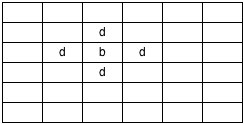
\includegraphics[width=\textwidth]{type1}
    \caption{Type-1 Neighborhood}
    \label{fig:type1}
  \end{subfigure}
  \begin{subfigure}[b]{0.4\textwidth}
    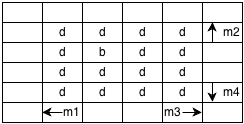
\includegraphics[width=\textwidth]{type2}
    \caption{Type-2 Neighborhood}
    \label{fig:type2}
  \end{subfigure}
  \caption{NPSF Neighborhoods \\
           b: base cell \\
           d: deleted neighborhood} 
           %$m_1$ = $m_2$ = 1; $m_3$ = $m_4$ = 2}
  \label{fig:npsftypes}
\end{figure}

Three classes of NPSF faults exist:
\begin{enumerate}
  \item Active NPSF (ANPSF): the base cell's contents change due to changes in the pattern of the deleted neighborhood.
  \item Passive NPSF (PNPSF): the base cell's contents cannot change due to specific pattern in the deleted neighborhood.
  \item Static NPSF (SNPSF): the base cell's contents are forced to a specific value because of the contents of the deleted neighborhood
\end{enumerate}

To test for all three classes of NPSF faults, all the combinations of values in the deleted cells and their transitions must be performed against the base cell.  To do this, a Eulerian Sequence is employed to generate the appropriate sequence of values in the neighborhood.  \cite{1675556} offers a proof of the Eulerian Sequence as a testing mechanism.  A 5-bit Eulerian Sequence is used as the Type-1 pattern.

To reduce the number of write operations to memory, multiple patterns can be written to memory simultaneously using either the tiling or two-group methods as shown in Figure \ref{fig:type1methods}.

\begin{figure}[h]
  \centering
  
\includegraphics[width=\textwidth]{placeholder}
  \caption{Type-1 with tiling method and two-group method}
  \label{fig:type1methods}
\end{figure}

In the tiling method, each tile is written to memory is such a way that none of the tiles overlap.  The two-group method is comprised to two checkerboard patterns that are overlaid is such a way that a base cell is in one checkerboard pattern while the deleted neighborhood is within the other checkerboard pattern.  This report will use the tiling method.

\section{Memory Test Algorithms}
\label{sect:bg-algorithms}
The early tests before the 1980`s were not based on fault models or proofs.  Tests of this time, such as Scan, GALPAT and Walking, were considered ad-hoc and usually have very long test times of order \textit{O(n\textsuperscript{2})} making the non-ideal for larger memories \cite{1327984}.  The introduction of fault models in the early 1980`s allowed the fault coverage to be mathematically proven.  This paved the way for March tests to become the dominant type of tests since their fault coverage is proven mathematically and test time is linearly related to the size of the memory \cite{1327984}.  

\subsection{GALPAT and variations}
The GALPAT or Galloping 1’s and 0’s algorithm sequences through all memory addresses to test for faults.  It starts by writing a background of zeros into all memory cells, then complements the first cell and compares it to every other cell, reading the base and test cell every time.  The test continues testing every cell by complementing the current cell and comparing it to every other cell \cite{oldref-09}.  The test is effective for finding stuck-at faults, coupling faults and transition faults, but suffers from an extremely long test time compared to march tests \cite{1327984}.  


\subsection{Walking Algorithms}
Walking algorithms are similar to GALPAT tests.  They begin by initializing all memory to zeros and then complement the first test cell, or base cell.  The test reads the base cell and then reads each of the memory cells to compare results without re-reading the base cell.  The test is effective at finding SAF, but suffers from test times proportional to \textit{O(n\textsuperscript{2})} \cite{VanDeGoor1991}.  


\subsection{March Test}
The March test has become the most popular testing algorithm for memory.  The March test algorithm is a finite sequence of March Elements (ME), each of which can be shared between other algorithms.  A ME specifies the sequence of actions, or March operations (MO), applied to each cell before proceeding to the next cell \cite{199799}.  The MO is the action performed at the memory cell: write a 0 (w0), write a 1 (w1), read a zero (r0) and read a 1 (r1) \cite{199799}.

The order in which the memory addresses are tested is the address order (AO), and the actual sequence of addresses is the counting method (CM).  For example, for the range 1\ldots10, the sequence 1,2,3,\ldots,9,10 would have an ascending AO and linear CM.  Conversely, 10,9,\ldots,3,2,1 would have a descending AO and a linear CM. The AO uses the symbols $\Uparrow$ (ascending),$\Downarrow$ (descending),$\Updownarrow$ (AO irrelevant) as abbreviations in the ME definition \cite{199799}.

The ME ‘$\Updownarrow$(r0,w1)’, is interpreted at each memory address as read the memory with expected value of \textit{0}, write a value of \textit{1} and continue to the next address in ascending order \cite{5491773}.    









\section{Memory Address Counting Methods}
\label{sect:bg-counting}
For any number \textit{N}, there are \textit{N}! ways to count to \textit{N}.  The memory address counting methods are important because they can directly affect a test's effectiveness at detecting faults.  Running the test with all possible CM (\textit{N}!) is not practical with today's memory sizes, so designers must use innovative CM that reduce test time while achieving maximum test coverage.  The address generator in this report will focus on CM that are common and important.  Each of the CM included has its own fault detection capability \cite{1347645}, \cite{990255}, \cite{1584048}, \cite{5359299}, \cite{1576336}.  Table \ref{tab:cm} provides an example of each CM for a four-bit address line.

\begin{table}[H]
  \caption{Address Counting Methods}
  \centering
  \begin{tabular}{|c|c|c|c|c|c|}
  \hline
  %heading
  Step & LI & AC   & GC & 2\textsuperscript{\textit{i}}=4 & PR \\
  \hline\hline
   0 & 0000 & 0000 & 0000 & 0000 & 0000 \\ 
   1 & 0001 & 1111 & 0001 & 0100 & 0001 \\ 
   2 & 0010 & 0001 & 0011 & 1000 & 0011 \\ 
   3 & 0011 & 1110 & 0010 & 1100 & 0111 \\ 
   \hline
   4 & 0100 & 0010 & 0110 & 0001 & 1111 \\ 
   5 & 0101 & 1101 & 0111 & 0101 & 1110 \\ 
   6 & 0110 & 0011 & 0101 & 1001 & 1101 \\ 
   7 & 0111 & 1100 & 0100 & 1101 & 1010 \\ 
   \hline
   8 & 1000 & 0100 & 1100 & 0010 & 0101 \\ 
   9 & 1001 & 1011 & 1101 & 0110 & 1011 \\ 
  10 & 1010 & 0101 & 1111 & 1010 & 0110 \\ 
  11 & 1011 & 1010 & 1110 & 1110 & 1100 \\ 
   \hline
  12 & 1100 & 0110 & 1010 & 0011 & 1001 \\ 
  13 & 1101 & 1001 & 1011 & 0111 & 0010 \\ 
  14 & 1110 & 0111 & 1001 & 1011 & 0100 \\ 
  15 & 1111 & 1000 & 1000 & 1111 & 1000 \\ 
   \hline
   \end{tabular}
   \footnotetext{Note: LI=Linear; AC=Address Complement; GC=Gray Code; PR=Pseudo-Random}
   \label{tab:cm}
\end{table}

\subsection{Linear Sequence}
The linear (LI) sequence CM is the standard numerical sequence.  Adjacent addresses differ by one numerical value.  The up `$\Uparrow$` sequence is 0, 1, 2, 3, \ldots, 2\textsuperscript{\textit{N}}-1 while the down `$\Downarrow$` sequence is 2\textsuperscript{\textit{N}}-1, \ldots, 3, 2, 1, 0.  Single-cell and coupling faults can be detected with this CM \cite{5941430}.

\subsection{Address Complement}
Address complement (AC) CM specifies an address sequence where pairs of addresses are formed using the address and its one's complement.  A four-bit address sequence would be: 0000, \textbf{1111}, 0001, \textbf{1110}, 0010, \textbf{1101}, etc \cite{VanDeGoor1991}.  In this series, the \textit{even steps} form a linear sequence while the \textit{odd steps} (in \textbf{bold}) are formed with the one's complement of its corresponding even pair.  This CM forces all bits to change in a transition between pairs and causes large amounts of noise, large power surges and maximum delay; it is ideal for detecting speed-related faults \cite{5941430}.

\subsection{Gray Code}
Gray code (GC) is a binary numbering system where successive values differ by only one bit \cite{VanDeGoor1991}.  In the context of memory addressing, the address transitions will differ only in one bit (i.e., they have a \textit{Hamming distance} of 1).  This CM produces minimal noise, power and delay and is used for the minimal stress tests \cite{5941430}.

\subsection{Worst-Case Gate Delay}
Speed related faults can be detected with the worst case gate delay (WCGD) CM.  For every address, the WCGD CM creates \textit{N} address-triplets consisting of the original address, the original address with a single bit inverted, and the original address again.  The address-triplets in WCGD CM have a \textit{Hamming} distance of 1 \cite{5359299}.  The WCGD CM is not implemented in the proposed design, but it described here for reference.

\subsection{2\textsuperscript{\textit{i}} Sequence}
2\textsuperscript{\textit{i}} CM uses address pairs that differ in \textit{one} bit.  The \textit{i} value specifies the numerical difference between two pairs of numbers and \textit{i} also specifies the bit that will be incremented or decremented.  For example, when \textit{i} = 3, 2\textsuperscript{3} = 8, so all address pairs in this sequence will vary by the bit 3, or by a value of 8.  This is a popular CM used to detect speed-related faults, especially in the Moving Inverions (MOVI) test \cite{5941430}.

\subsection{Pseudo-Random}
A pseudo-random (PR) CM generates a sequence of addresses that appear to be random, but are deterministic and can be reproduced.  These sequences are commonly generated using an LFSR which implements a characteristic polynomial function \cite{VanDeGoor1991}.  



\section{Challenges in Testing Embedded Memory}
\label{sect:bg-challenges}

\subsection{At-Speed}
To effectively detect memory faults, the test must be run at least at the maximum operating clock frequency for the memory device.  At-speed testing is important because timing for the chip may only be closed at “limited” test corners or external testing at high speed may be difficult or even impossible.  Transition faults may not be detected if the chip is run below maximum operating frequency \cite{1583992}.  

\subsection{Back-to-Back (BtB) Access}
Back-to-Back (BtB) accesses are necessary to detect faults that may occur when an action is repeated on a memory cell.  BtB means the CPU uses the smallest number of clock cycles to access memory \cite{5491773}.  One fault that may only present during BtB testing is a cell suffering from read disturbance and losing its charge after 16 consecutive reads \cite{4079351}.  The faults are subtle enough that external testing may not be able to detect is the correct sequence or repetitions is not executed.  Detecting these types of faults requires augmenting existing March test algorithms to effectively screen parts.  

\subsection{Area}
The area cost of MBIST circuits is usually small compared to the memory under test, but for an SoC consisting of hundreds of memory cores \cite{4711617} or programmable memory BIST with a large amount of instruction memory \cite{5692281}, the area overhead for the BIST circuits will be very high.  To continue Moore’s law and maintain acceptable yields with the larger memory sizes, the BIST circuits will require innovation to reduce their footprint.

\subsection{Power}
Power dissipation during the MBIST is an important challenge because of the problems that may occur.  High power during test along with the high switching frequency can cause excessive noise that can change the state of a circuit and cause a good die to fail the test and reduce yield \cite{oldref-15}, or cause circuit damage and destroy the chip \cite{oldref-16}, again reducing yield.



\section{Designs to Address Challenges}
\label{sect:bg-designs}
MBIST is a hot-topic due to its increased importance in the new memory-dense SoCs.  The challenges with the current MBIST topologies are well known.  New innovations and design methods have been introduced to overcome these obstacles.

\subsection{Topologies}
There are three types of BIST topologies commonly used: finite state-machine (FSM)-based designs, micro-programmable based designs and microcode-based designs.  Each has advantages and disadvantages that designers must consider to meet the requirements of their product. 

\subsubsection{FSM-Based Designs}
In FSM-based designs, the control signals for the BIST are defined as state machines and are usually hardwired, or non-programmable.  The FSM-based topology benefits from having a smaller area, but lacks flexibility to change its algorithm to support new fault models without redesign of the chip \cite{5692281}.  New FSM-based designs are beginning to incorporate some level of programmability, but at the cost of area \cite{4815717} or clock frequency and test time \cite{748806}.

\subsubsection{Micro-Programmable-Based Designs}
The micro-programmable-based designs use a microprocessor to generate the algorithm.  These designs have high flexibility with their algorithms, but in-turn require a high area overhead for the processor \cite{726568}.  Additionally, this type of design is not well suited for a stand-alone embedded RAM intellectual property (IP) core because of the processor requirement \cite{1584083}.

\subsubsection{Microcode-Based Designs}
Microcode-based topologies use written sets of instructions that are loaded into memory to execute memory test patterns.  The controllers for microcode-based topologies are designed as programmable MBIST with the flexibility to select any instructions from supported set of test instructions.  The test flexibility and ability to reprogram this design allows it to easily support new fault models should a test escape be discovered.  The flexibility comes at a cost though in the storage area for the microcode instructions \cite{5692281}, \cite{114099}.  The area overhead is a carefully evaluated intensively during the selection of the BIST design. 

\subsection{Existing Designs}
The following section examines some of the state-of-the-art design methods and innovations currently being explored to address the MBIST implementation challenges.  In general, at-speed challenges and to a lesser extent BtB have mostly been addressed by using MBIST to test memories, but area and power challenges still exist which and are being actively researched.  The following section focus on BtB accesses, area reduction and power reduction in MBIST as they are the leading topics of research for MBIST improvements.

\subsubsection{Design Methods for At-Speed and BtB Access Challenges}
Even with the use of MBIST, BtB testing presents a particularly difficult problem because the architecture of the CPU and its interactions with the memory controller must be well understood.  Memory failures are now more frequently caused by speed-related faults rather than static faults.  To screen for these faults, a test must be able to access memory as fast as the CPU.  The design proposed in \cite{5491773} addresses this issue by using the CPU’s assembly language and core to test the memory.

In \cite{5491773}’s proposed solution, a small set of the assembly instructions for basic memory movement and logical functions are used to write March test algorithms.  Memory interleaving, or folding, is also addressed in the new algorithms.  The algorithms satisfy the BtB test requirements mainly by variations of loop-unrolling or by coding tight jump loops that still allow BtB memory access.     

\subsubsection{Design Methods for Area Challenges}
Area is generally a concern for chips with multiple memory cores or with microcode-based designs that offer high flexibility.  One potential solution \cite{4711617} to reducing the area used by multiple memory cores is a pipelined MBIST for homogeneous RAMs.  The paper identifies the test pattern generator as a significant portion of the BIST area proposes to use only one generator.  It accomplishes this sending the pattern to the first memory, then uses the output of the first memory as the input to the second memory effectively pipelining the BIST and reducing the area overhead.  The test controller still manages the memory selects, addressing and data verification, but only needs to control one pattern generator which also reducing wire routing area.

Another approach to reduce the MBIST footprint is to optimize the microcode itself \cite{5692281}.  This design takes advantage of the fact ME repeat for various algorithms and furthermore, usually show up in repeated clusters.  These clusters are identified and defined as macros, and then the macros are encoded as new microcode instructions.  So effectively, a group ME instructions has now become one microcode instruction.  The solution is similar to creating a library function in software where it only physically resides in one memory location rather than at each invocation of the function.  

\subsubsection{Design Methods for Power Challenges}
MBIST power is a concern because it is generally higher than normal operating power and it can have negative effects on yield.  Novel techniques to optimize blocks of the MBIST help to reduce average and peak power usage.  One technique \cite{oldref-15} proposes a low power linear feedback shift register (LFSR) for the test pattern generator (TPG).  This paper targets switching activity in the LFSR as one culprit for higher power - in particular, the non-correlated patterns cause higher power dissipation.  The paper proposes using intermediate transitional vectors.  In between two successive vectors, half of the first pattern is changed and output, then the second half is changed and output, then a few logic gates are added to generate a third output before finally outputting the new pattern.  With this piecewise technique, five test patterns are generated while only using power equal to generating two vectors.

The previous proposal showed how optimizing the pattern generation could reduce power.  The next paper discusses ways to optimize the address generation block used for March tests by reducing switching activity.  The following sequence is typically used for testing stuck-at faults:
⇕(w0), ⇕(r0), ⇕(w1), ⇕(r1) 
This sequence results in a large amount of switching activity in the address decoder.  The paper proposes to instead use this pattern to reduce the activity:

⇕(w0, r0, w1, r1)

The address decoder now only needs to change once per memory address while the stuck-at faults can still be detected.  The paper further suggests alternate LFSR designs which offer better correlation between bit patterns.  Patterns that are reduce the actual number of bits that change will reduce the switching activity.  The Bit-Swapping LFSR (BS-LFSR) swaps values between neighboring bits and reduces switching activity by about 25\% \cite{4472405} while the Bipartite LFSR reduces switching activity by combining the first and second halves of the current vector with the next vector to create intermediate vectors \cite{oldref-03}.    






\chapter{Proposed Design}
\label{chap:design}

The design in this report is based upon \cite{1584083} which proposes a programmable memory BIST with auxiliary memory for NPSF.  This design will modify the programmable memory BIST by introducing a pattern generator to dynamically generate the NPSF Type-1 neighborhood patterns.  It will also replace the address counter with a programmable address generator to allow more flexibility in testing specific addresses sequences.

\section{PMBIST Hardware Blocks}
\label{sect:bg-blocks}
The proposed design is comprised of five major blocks: the scan and instruction register; the cycle controller; the address generator block; the data generator and compare block; and the operation control block;.  The major blocks and their connections are illustrated in Fig. \ref{fig:pmbistall} and the following sections descibe the blocks in more detail.

\begin{figure}[h]
  \centering
  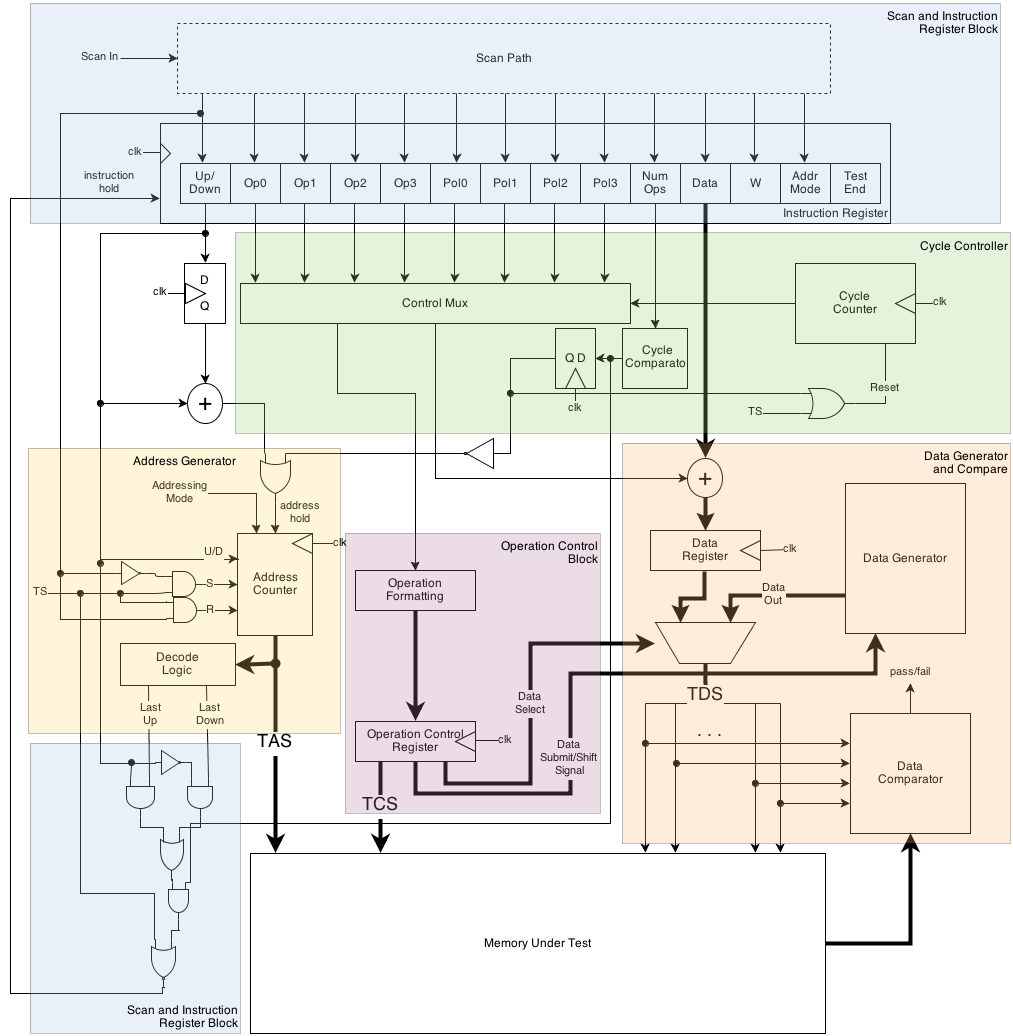
\includegraphics[scale=0.4]{pmbistall}
  \caption{Major Block of the PMBIST Design}
  \label{fig:pmbistall}
\end{figure}

\subsection{Cycle Controller}
The cycle controller determines which march operation should execute on the current address.  When all march operations have completed on the current address, the cycle controller generates a signal that allows the address counter to move to the next test address.  The cycle controller then resets the march operation pointer to the first operation for the next address.   

\subsubsection{Control Mux}
The control mux receives all the operation and polarity signals from the instruction register.  Using the cycle counter's output as the mux control signal, the control mux selects the operation and polarity signal corresponding to the current cycle and outputs them to the operation formatting block and control register.  

\subsubsection{Cycle Counter}
The cycle counter increments the count for the march operation to execute.  The output of the cycle counter corresponds to the active march operation.  The cycle counter is incremented by the clock signal and can be reset by a TS signal or when the current march sequence has completed for the current memory address. 

\subsubsection{Cycle Comparison}
The cycle comparison unit compares the current cycle to the NO field of the instruction register.  When the cycle counter matches the NO field, the comparison block generates an active high signal that is stored in the cycle controller's local flip-flop.  The signal is also sent to the instruction register hold logic block.  

\subsection{Address Generation}
The memory address to test and memory control signals are generated by the address and operation block.  The address decode block is used to generate the instruction register hold signal.  The hold signal maintains the instruction register's data until the current march sequence has completed for all memory address.  

\subsubsection{Address Counter}
The address counter indicates the memory address to test.  The direction of the address order can be programmed to increment or decrement through memory.  The order of addresses is also programmable: linear up/down, pseudo-random sequence using LFSR, address complement, Gray coding, and 2\textsuperscript{i} counting methods.
 
\subsubsection{Address Decode Logic}
The address decode logic block determines if the address generated by the address counter is the last up (LU) or last down (LD) memory address for the current march sequence.  The decode logic uses the signals from the address programmer block to determine whether the sequence direction is up or down.   

\subsection{Operation Control Block}
In some designs, the memory algorithm operation signals from the instruction register do not necessarily need to match the memory's control signals.  The operation formatting block can be used to translate the instruction register's operation code to the memory controller's signals such as write/read, enable and reset.

\subsubsection{Operation Formatting}
The Operation Formatting block converts the memory algorithm operation signal to explicit memory control signals such as read/write, enable and reset.  The output of this block passes to the control register.

\subsubsection{Operation Control Register}
The control register interprets the operation formatted instruction and sends any internal control signal to other blocks of the PMBIST.  In particular, this block sends the data mux select signal and controls the sequencing of the data generator.  It also writes the memory control signals to the TCS bus.  

\subsection{Data Generator and Compare}
Data can come from the instruction register or the data generator.  A mux select signal is generated based on the current operation.  For user data patterns, the data from the instruction register is selected and written to memory.  For NPSF patterns, the data generator outputs the word to be written to memory.  The comparator checks if the data read from memory matches what is expected and generates the pass/fail signal.

\subsubsection{Data Generator}
\begin{figure}[h!]
  \centering
  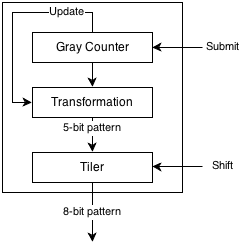
\includegraphics[scale=0.5]{datagen}
  \caption{Data Generator Block Diagram}
  \label{fig:datagen}
\end{figure}
The data generator block design is shown in \ref{fig:datagen}.  The gray counter is a 5-bit counter that generates gray code and repeats after 32 iterations.  The gray code is passed to the transform block which converts the code to a Eulerian Sequence.  A detailed description of the Euler Sequence can be found in \cite{1675556}.  Essentially, a 5-bit Euler Sequence used as the Type-1 NPSF background will transition through all the possible read and write combinations that could occur.  This requires 161 different sequences which can be broken into five groupings as shown in \ref{tab:euler}.  Except for the first column, each column is generated by a one-bit right shift and rotate followed by inverting the most and least significant bits \cite{00957583}.

\begin{table}[h]
  \caption{Partial 5-bit Euler Sequence}
  \centering
  \begin{tabular}{c c c c c c}
  \hline\hline
  Iteration    & Gray (E[0]) & E[1]  & E[2]  & E[3]  & E[4]  \\
  X0  & 00000 & 10001 & 01001 & 00101 & 00011 \\
  X1  & 00001 & 00001 & 00001 & 00001 & 00001 \\
  X2  & 00011 & 00000 & 10001 & 01001 & 00101 \\
  ......             & ...   & ...   & ...   & ...   & ...   \\
  X29 & 10011 & 01000 & 10101 & 01011 & 00100 \\
  X30 & 10001 & 01001 & 00101 & 00011 & 00000 \\
  X31 & 10000 & 11001 & 01101 & 00111 & 00010 \\ [0.5ex]
  \end{tabular}
  \label{tab:euler}
\end{table}

The transformation block provides the 5-bit Euler Sequence to be used as the NPSF background.  To write this value to memory using the Type-1 tiling method, the sequence must be spread over the adjacent rows to create the correct tiling background as shown in \ref{fig:tiling}.  

\begin{figure}[h!]
  \centering
  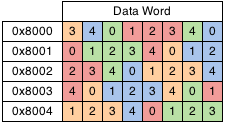
\includegraphics[scale=0.5]{type1tiling}
  \caption[Type-1 Neighborhood Tiling Method for Design]{Type-1 Neighborhood Tiling Method for Design}  
   Each 5-bit color block represents one Type-1 neighborhood.
  \label{fig:tiling}
\end{figure}

\subsubsection{Data Comparator}
Each read march element is checked with the data comparator.  The comparator accepts as inputs the TDS bus and the output of the MUT.  If the MUT output matches the TDS value, a pass signal is generated.  If there is any discrepancy, the fail signal is generated.  

\subsubsection{Polarity and Data Register}
The polarity signal from the current march operation is used to invert the data.  If the polarity signal is false (0), the data is unmodified and stored to the data register.  If the polarity signal is true (1), the data is inverted, then stored in the data register.  

\subsection{External Connections}
Integration with the MUT and scan-path requires a few external connections.  The scan-path writes data to the instruction register for the test.  The MUT receives address, data and control signals from the memory BIST.

\subsubsection{Scan-Path Connection}
The scan-path receives data serially for the memory BIST.  The scan-path signals correspond to the instruction register fields.  When the scan-in data has been clocked into place, the instruction register will latch the data and begin its test.  

\subsubsection{Memory Under Test Connections}
The MUT connects to the MBIST through the test buses.  The connections provides the data, control signals and address to the memory and are connected to the memory input pins.  

\paragraph{Test Address Signals}
The test address signals (TAS) compose the memory address currently on interest to the test.  They can point to the read address for a comparison or check or the write address to store new data.

\paragraph{Test Control Signals}
The test control signals (TCS) are generated from the instruction register's operation field.  The signals are formatted to work with the MUT.  The opcode is translated to the memory control signals such as read/write, reset and enable.  

\paragraph{Test Data Signals}
The test data signals (TDS) contain the data to be stored in memory.  These signals are connected to the MUT's data input pins and the data comparator's input pins.  They are driven from the data register.  When an auxiliary memory is used, the data pins are driven from the outputs of the auxiliary memory.


\section{Modifications to Programmable MBIST}
\label{sect:bg-modifications}
These modifications were made to the design.

\subsection{Address Generator Expansion}
The address generator originally supported linear and pseudo-random address counting methods.  The design in this report will add Gray code, address complement and 2\textsuperscript{i} counting methods.

\subsection{Programmable Address Generator}
The original design did not make use of the address mode field and left it to the designer to decide on whether to implement the psuedo-random or linear counting methods.  The only programmability for address was the direction which was set using the up/down field.  This report adds the ability to select which address generation pattern to use.  The instruction register was expanded with new fields for address generation modes to allow programmability, and the instruction field is decoded within the BIST to select the address counting method.

\begin{table}[hbt]
  \caption{PMBIST Address Modes}
  \centering
 \begin{tabular}{|p{1in}|p{0.75in}|p{3in}|}
  \hline
  Name & Op Code (binary) & Description \\ [0.5ex]
  \hline\hline
  Linear              & 0000 & Standard numerical sequence  \\ 
  \hline
  Pseudo-Random       & 0001 & Repeatable random sequence \\ 
  \hline
  Address \ Complement  & 0010 & Progresses linearly on even steps and inverts all bits on odd steps.\\ 
  \hline
  \textit{Reserved}            & 01XX & Available for additional addressing modes \\ 
  \hline
  Gray Coding         & 0011 & Changes only one bit per address transistion \\ 
  \hline
  2\textsuperscript{\textit{i}}& 1[j\textsubscript{2:0}] & Generates all address pairs with a \textit{Hamming} distance of 1.  2\textsuperscript{\textit{i}} = \textit{j}\textsubscript{2:0} where \textit{i} is the address bit that determines address-pair for \textit{Hamming} distance. \\ 
  \hline
 \end{tabular}
\label{tab:addrmode}
\end{table}

\subsection{Dynamic Background Pattern Generation}
The auxiliary memory is used to store NPSF background patterns in the base design.  To reduce the area required by this design, the auxiliary memory is replaced by a dynamic background pattern generator.  The generator creates the Type-1 neighborhood pattern and translates it to an 8-bit value that can be written sequentially to memory to create the background pattern.





\chapter{Results}
\label{chap:results}
The design results are presented in this section.  The design was compiled using Synopsys Design Compiler with the Artisan 45nm typical libraries.  The area measurements are taken from Design Compiler's built-in area report generator.  The memory size information is obtained for Artisan Memory Compiler tools using the 180nm library.  To show a more accurate comparison, the area from the Memory Compiler tool has been scaled to a more comparable size.  This does not affect the analysis as the memory area is only used as a value to reference the orignal BIST and proposed BIST designs.  

\section{Area Comparisons}
This report shows how a robust address and pattern generation scheme can be implemented with very little increase in area.  The implementation does require some additional area over the base design.  For large memory blocks, the address generator only requires 0.6\% more area overhead than the base design.  Similarly, the pattern generator adds 1.0\% more area within the memory block.  For designs using an auxiliary memory, the pattern generator reduces the overall memory area by 50\%.  

\label{sect:cln-area}
\subsection{Address Generator Area}
The original base design only offered binary and LFSR up/down counters for address counting methods.  The proposed design improves on the base design by providing a more robust address counting method that industry uses to test memory during production.  Table \ref{table:ac_area_compare} below shows the area increases by  59.3\% for the address counter block and 17.7\% for the overall PMBIST area.  

\begin{table}[ht]
\caption{Address Counter Area (\textit{um\textsuperscript{2}})}
\centering
\begin{tabular}{| l | l | l | l |}
\hline
Component & Base Design & Proposed Design & Percentage Difference \\ [0.5ex]
\hline\hline
address counter & 1810   & 2884   & 59.3\% \\
pmbist area     & 6057   & 7132   & 17.7\% \\ 
\hline
\end{tabular}
\label{table:ac_area_compare}
\end{table}

It is important to note the overall area difference with respect to the full memory block.  This can be interpreted as the area cost for the additional address counting methods that ease manufacturing tests and add more robustness to the PMBIST.  Table \ref{table:ac_area_overhead} shows the percentage of the total memory block used by the original and proposed address counter designs.  As the memory sizes increase, the area increase due to the address generator becomes insignificant when the benefits of the new addressing schemes are considered.   

\begin{table}[ht]
\caption{Address Counter Area within Memory Block}
\centering
\begin{tabular}{p{0.5in} p{1.25in} | l | l | l |  }
\cline{3-5}
& & \multicolumn{3}{ c| }{Area Overhead Percentages} \\
\hline
\multicolumn{1}{|p{0.5in}|}{Memory Size} & Total Memory Area (\textit{um\textsuperscript{2}}) & Base Design & Proposed Design & Difference \\ [1ex]
\hline\hline
\multicolumn{1}{|c|}{64x8  }  & 15780  & 27.7\% & 31.1\% & 3.4\% \\
\multicolumn{1}{|c|}{128x8 }  & 16884  & 26.4\% & 29.7\% & 3.3\% \\
\multicolumn{1}{|c|}{256x8 }  & 19333  & 23.9\% & 26.9\% & 3.1\% \\
\multicolumn{1}{|c|}{512x8 }  & 24108  & 20.1\% & 22.8\% & 2.7\% \\
\multicolumn{1}{|c|}{1024x8}  & 34013  & 15.1\% & 17.3\% & 2.2\% \\
\multicolumn{1}{|c|}{2048x8}  & 53276  & 10.2\% & 11.8\% & 1.6\% \\ 
\multicolumn{1}{|c|}{4096x8}  & 92093  & 6.2\%  & 7.2\%  & 1.0\% \\
\multicolumn{1}{|c|}{8192x8}  & 172577 & 3.4\%  & 4.0\%  & 0.6\% \\ [1ex]
\hline
\end{tabular}
\label{table:ac_area_overhead}
\end{table}


\subsection{Pattern Generator Area}
The pattern generator offers a built-in solution to replace auxiliary memories used for NPSF Type-1 tiling neighborhoods.  Table \ref{tab:pg_memory_compare} shows the estimated area for small memories that may be used for auxiliary memory to store patterns.  This table shows the pattern generator uses 78.6-90.4\% less area than the auxiliary memory.  With such a large area reduction, additional circuits to generate other patterns could be added and still use less area than an auxiliary memory.

\begin{table}[h]
\caption{Area of Pattern Generator Compared to Auxiliary Memory}
\centering
\begin{tabular}{|c| c| c|}
\hline
Memory Size & Memory Area & Area Reduction \\ [0.5ex]
\hline\hline
4x8   & 10289 & 78.6\%  \\
8x8   & 11393 & 80.6\%  \\
16x8  & 12497 & 82.4\%  \\
32x8  & 13601 & 83.8\%  \\
64x8  & 14706 & 85.0\%  \\
128x8 & 15809 & 86.0\%  \\
256x8 & 18258 & 87.9\%  \\
512x8 & 23033 & 90.4\%  \\
\hline
\end{tabular}
\label{tab:pg_memory_compare}
\end{table}

For designs using an auxiliary memory to store NPSF Type-1 tiling neighborhoods, the pattern generator will actually reduce PMBIST memory overhead for memory.  Table \ref{tab:pg_memory_overhead} shows the total memory block area can decrease by 5.0-35.2\% when an 8x8 auxiliary memory is replaced by the pattern generator.  

\begin{table}[h]
\caption{Pattern Generator Memory Area Reduction}
\centering
\begin{tabular}{|c| c| c| c| c|}
\hline
Memory Size & Base Design & with Aux. Mem & with PG & Area Reduction \\
\hline\hline
64x8   & 14706  & 26099  & 16911  & 35.2\% \\
128x8  & 15809  & 27202  & 18015  & 33.8\% \\
256x8  & 18258  & 29651  & 20464  & 31.0\% \\
512x8  & 23033  & 34426  & 25239  & 26.7\% \\
1024x8 & 32939  & 44332  & 35144  & 20.7\% \\
2048x8 & 52202  & 63595  & 54407  & 14.4\% \\
4096x8 & 91019  & 102412 & 94224  &  9.0\% \\
8192x8 & 171503 & 182896 & 173708 &  5.0\% \\ [0.5ex]
\hline
\end{tabular}
\label{tab:pg_memory_overhead}
\end{table}

\subsection{Address and Pattern Generator within Memory Block}
Combining the address and pattern generator will provide the most flexibility with the memory test algorithm while also minimizing the increase in the memory area to accommodate the new features.  While the address generator adds to the total area, combining it with the pattern generator's area reduction actually achieves a better area than the original base design with a simple address counter and auxiliary memory.  Figure \ref{fig:all_compare} shows the area reduction achieved by combining both the address and pattern generator.

\begin{figure}[h]
  \centering
  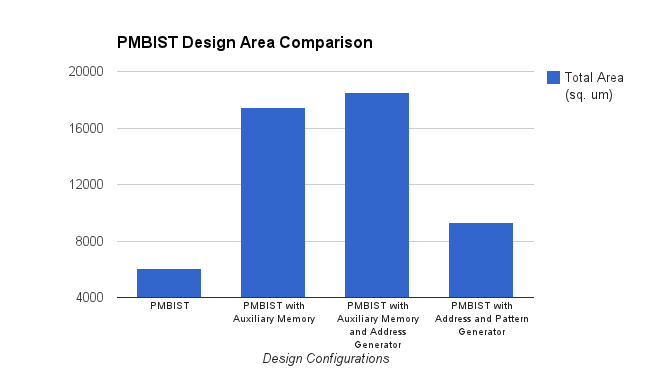
\includegraphics[width=\textwidth]{PMBIST_compare}
  \caption{Area Comparison of Different PMBIST Configurations}
  \label{fig:all_compare}
\end{figure}

Compared to the original base design, the design implemented in this report achieves a more robust address generation scheme while using less area than the original design thanks to the use of a pattern generator in place of an auxiliary memory.  As a final comparison the memory overheads for the various PMBIST designs discussed in this report are presented in Table \ref{tab:all_overhead}.  This table shows the percentage of the total memory IP block used by each of the PMBIST designs.  The design with combined address and pattern generation only increases the memory overhead by 1.8-9.6\% depending on memory size.  By comparison, the designs using auxiliary memory add an additional 6.3-26.5\% area overhead to the design.  

\begin{table}[h]
\caption{Area Overhead Added by PMBIST Designs}
\centering
\begin{tabular}{|p{0.75in}| p{0.6in}| p{0.9in}| p{0.9in}| p{0.6in}|}
\hline
Memory Size & Base Design & Base with Aux. Mem. & AG with Aux. Mem. & AG with PG  \\
\hline\hline
64x8   & 29.2\% & 54.3\% & 55.7\% & 38.8\% \\
128x8  & 27.7\% & 52.5\% & 54.0\% & 37.1\% \\
256x8  & 24.9\% & 48.9\% & 50.4\% & 33.8\% \\
512x8  & 20.8\% & 43.1\% & 44.6\% & 28.8\% \\
1024x8 & 15.5\% & 34.6\% & 36.0\% & 22.1\% \\
2048x8 & 10.4\% & 25.1\% & 26.2\% & 15.2\% \\
4096x8 &  6.2\% & 16.9\% & 16.9\% &  9.3\% \\
8192x8 &  3.4\% &  9.7\% &  9.7\% &  5.2\% \\ [0.5ex]
\hline
\end{tabular}
\label{tab:all_overhead}
\end{table}








\chapter{Conclusion}
This chapter summarizes the results and discusses future work for this design.
\section{Discussion}
This work presented the initial design stages of a SAR-based pipeline ADC. With ever increasing focus on portable applications, power efficiency in ADCs will only become more important in the future. SAR ADCs are well known to be power efficient for applications requiring low sampling rates and medium to high resolutions. Applying the principles of pipelined ADCs to a SAR topology can increase the SAR application space to medium speed applications while still maintaining the power efficiency and high accuracy of the SAR topology. This design used a half-gain MDAC topology in order to reduce the required output swing and to increase overall ADC linearity. The half-gain topology alowed for the use of a triple-cascode OTA, which ended up being a low current solution. A novel scheme to obtain an additional bit of accuracy without increasing capacitance by utilizing the dummy LSB capacitor was also implemented. Although ideal clocks, comparators, and switches were used the OTA performance generally dominates the power and SNDR figures. The total figure of merit obtained from this design show that this topology has a lot of promise for power constrained designs.
\section{Future Work}
While this design covers the majority of the implementation of the ADC, there is still much to be done to ensure that this design would perform adequately when taped out. Some additional architectural modifications could reduce the load capacitance of the design signficantly. In addition, there are circuit level optimizations that could be performed on both the OTA and the digital control logic. Finally, some additional blocks need to be designed and additional simulations need to be performed. 

An extension of the implementation scheme in \ref{sec:dummylsbarch} could be used to obtain an additional bit of accuracy, or alternatively to halve the load capacitance in the second stage. Additionally, the differential scheme produces an additional bit of resolution that is currently not being utilized. This could lead to a factor of four reduction in load capacitance from the second stage capacitors. This could result in reduced power consumption or an increased sampling rate. These facts, along with realistic data on the parasitics from the OTA, suggest some re-architecting of the design could be done. The resolution of the two stages can be adjusted in order to achieve the best balance between sampling rate, power consumption, and total resolution. Furthermore, one large issue with the OTA design is that it will not scale well to future lower voltage processes. A reevaluation of the OTA topology used would like be a worthwhile exercise as well. Performing these architectural modifications could greatly improve the total performance of the design.

One disadvantage to the usage of the implementation scheme in \ref{sec:dummylsbarch} is the additional reference voltages required to obtain the additional bit of accuracy from the dummy LSB capacitor. The voltages used in this report were ideal, so the additional reference voltages did not affect the overall power consumption of the design. This would not be true in a real design, however. Designing additional voltage references that are at least 12-bit accurate is a non-trivial task and the implementation may end up consuming too much power to be beneficial for the design. An alternative scheme that introduces some imbalance in the SAR common-mode voltage can be used to obtain the additional bit without introducing more reference voltages. This scheme could only be implemented in the second stage of the pipeline, because introducing this imbalance could cause inaccuracies in the residue voltage. This is not a severe disadvantage, however, since the second stage sampling capacitance has a larger effect on the OTA power consumption than the first stage capacitance. Adding an additional bit to the first stage through traditional means would mean an increase in total area, but since the unit capacitance of the first stage is not at its minimum this increase could be mitigated slightly. This is a limitation that could likely be overcome. 

In addition to the architectural modifications the OTA and digital control logic performance could likely be improved at the circuit level. The OTA performance could likely be improved by reducing the input capacitance to the amplifier. Another area worth taking a second look at is the digital control logic. Although the OTA dominates total power consumption, the switching of the SAR capacitors and the digital control logic contribute about 20\% of the power. The digital logic was designed at the gate level using standard cells. It may be worthwhile to transform this design into register-transfer level (RTL) code, such as Verilog. Once this transformation is complete, a synthesis tool could be used to try to reduce the power consumption of the digital control logic even further. 

After completing this front-end work, the clocking network, comparators, and switches will need to be designed. Simulations will need to be run on all these blocks both individually and integrated into the ADC to ensure that the ADC will meet its performance requirements across all process corners. Once all this work is done, a layout and parasitic extraction can be performed. With this data, additional simulations and design adjustments can be performed in order to obtain a high level of confidence that a manufactured design will meet its specifications. Finally, the design will need to be manufactured and tested. Depending on the results from this testing, additional debugging and design adjustments may be necessary to achieve the desired performance. In the ideal case, first silicon would yield the desired results, but if this is not the case another manufacturing run could be performed with an additional round of testing to follow. If all goes well in this second stage, working silicon could be demonstrated.

%%%%%%%%%%%%%%%%%%%%%%%%%%%%%%%%%%%%%%%%%%%%%%%%%%%%%%%%%%%%%%%%%%%%%%
% Appendix/Appendices                                                %
%%%%%%%%%%%%%%%%%%%%%%%%%%%%%%%%%%%%%%%%%%%%%%%%%%%%%%%%%%%%%%%%%%%%%%
%
% If you have only one appendix, use the command \appendix instead
% of \appendices.
%
%\appendices
%\index{Appendices@\emph{Appendices}}%

%\chapter{Lerma's Appendix}
\index{Appendix!Lerma's Appendix@\emph{Lerma's Appendix}}%
The source \LaTeX{} file for this document is no longer quoted in
its entirety in the output document. A \LaTeX{} file can 
include its own source by using the command
\cn{verbatiminput\{\cn{jobname}\}}.





%%%%%%%%%%%%%%%%%%%%%%%%%%%%%%%%%%%%%%%%%%%%%%%%%%%%%%%%%%%%%%%%%%%%%%
% Generate the bibliography.					     %
%%%%%%%%%%%%%%%%%%%%%%%%%%%%%%%%%%%%%%%%%%%%%%%%%%%%%%%%%%%%%%%%%%%%%%
%								     %
% NOTE: For master's theses and reports, NOTHING is permitted to     %
%	come between the bibliography and the vita. The command      %
%	to generate the index (if used) MUST be moved to before      %
%	this section.						     %
%								     %
%\nocite{*}      % This command causses all items in the 		     %
                % bibliographic database to be added to 	     %
                % the bibliography, even if they are not 	     %
                % explicitly cited in the text. 		     %
		%						     %
\bibliographystyle{plain}  % Here the bibliography 		     %
\bibliography{diss}        % is inserted.			     %
%\index{Bibliography@\emph{Bibliography}}%			     %
%%%%%%%%%%%%%%%%%%%%%%%%%%%%%%%%%%%%%%%%%%%%%%%%%%%%%%%%%%%%%%%%%%%%%%
%%%%%%%%%%%%%%%%%%%%%%%%%%%%%%%%%%%%%%%%%%%%%%%%%%%%%%%%%%%%%%%%%%%%%%
% Vita page.							     %
%%%%%%%%%%%%%%%%%%%%%%%%%%%%%%%%%%%%%%%%%%%%%%%%%%%%%%%%%%%%%%%%%%%%%%

%\begin{vita}
%\end{vita}

%%%%%%%%%%%%%%%%%%%%%%%%%%%%%%%%%%%%%%%%%%%%%%%%%%%%%%%%%%%%%%%%%%%%%%
% Generate the index.						     %
%%%%%%%%%%%%%%%%%%%%%%%%%%%%%%%%%%%%%%%%%%%%%%%%%%%%%%%%%%%%%%%%%%%%%%
%								     %
% NOTE: For master's theses and reports, NOTHING is permitted to     %
%	come between the bibliography and the vita. This section     %
%	to generate the index (if used) MUST be moved to before      %
%	the bibliography section.				     %
%								     %
%\printindex%    % Include the index here. Comment out this line      %
%		% with a percent sign if you do not want an index.   %
%%%%%%%%%%%%%%%%%%%%%%%%%%%%%%%%%%%%%%%%%%%%%%%%%%%%%%%%%%%%%%%%%%%%%%



\end{document}
